\documentclass[10pt,table,mathserif]{beamer}
\usetheme[
%%% options passed to the outer theme
%    hidetitle,           % hide the (short) title in the sidebar
%    hideauthor,          % hide the (short) author in the sidebar
%    hideinstitute,       % hide the (short) institute in the bottom of the sidebar
%    shownavsym,          % show the navigation symbols
%    width=2cm,           % width of the sidebar (default is 2 cm)
%    hideothersubsections,% hide all subsections but the subsections in the current section
%    hideallsubsections,  % hide all subsections
%    right                % right of left position of sidebar (default is right)
  ]{Aalborg}

\setbeamertemplate{theorems}[numbered]

\definecolor{watred}{cmyk}{.00,1,1,0.00}
\definecolor{watyellow}{cmyk}{0,0.12,1,0}
\definecolor{watgray}{cmyk}{0,0,0,0.5}

% If you want to change the colors of the various elements in the theme, edit and uncomment the following lines
% Change the bar and sidebar colors:
\setbeamercolor{Aalborg}{fg=black,bg=watred}
\setbeamercolor{sidebar}{bg=white}
% Change the color of the structural elements:
\setbeamercolor{structure}{fg=red}
% Change the frame title text color:
%\setbeamercolor{frametitle}{fg=blue}
% Change the normal text color background:
\setbeamercolor{normal text}{bg=white, fg=black}
\setbeamercolor{alerted text}{bg=white, fg=red}
% ... and you can of course change a lot more - see the beamer user manual.
\usepackage{xcolor}
\usepackage[utf8]{inputenc}
\usepackage[english]{babel}
\usepackage[T1]{fontenc}
\usepackage{threeparttable}
% ... or whatever. Note that the encoding and the font should match. If T1
% does not look nice, try deleting the line with the fontenc.
\usepackage{lmodern}
\usepackage{subcaption}
\usepackage{algorithm}
\usepackage{algorithmic}
\usepackage{colortbl}
\usepackage{biblatex}
\usepackage{bibentry}
\usepackage{epstopdf}
\usepackage{caption}
\usepackage{multirow}

\usepackage{tikz}
\usetikzlibrary{shapes}
\usetikzlibrary{arrows}
\usetikzlibrary{positioning, fit, arrows.meta}
\usepackage{tkz-graph}
\usetikzlibrary{backgrounds,automata}
\bibliography{mybib.bib}



\newcommand*{\Scale}[2][4]{\scalebox{#1}{$#2$}}%
\newcommand*{\Resize}[2]{\resizebox{#1}{!}{$#2$}}%
\newcommand{\vt}[1]{\mathbf{#1}}
\newcommand{\vw}{\mathbf{w}}
%\newcommand{\pm}{\stackrel{+}{-}}
\newcommand{\vx}{\mathbf{x}}
\newcommand{\vi}{\mathbf{i}}
\newcommand{\vo}{\mathbf{o}}
\newcommand{\vxt}{\tilde{\mathbf{x}}}
\newcommand{\vy}{\mathbf{y}}
\newcommand{\impsigma}{\breve{\sigma}}
\newcommand{\barK}{\overline{K}}
\newcommand{\barC}{\overline{C}}
\newcommand{\vz}{\mathbf{z}}
\newcommand{\fnp}{\tilde{f}}
\newcommand{\vu}{\mathbf{u}}
\newcommand{\vs}{\mathbf{s}}
\newcommand{\vc}{\mathbf{c}}
\newcommand{\E}{\mathbf{E}}
\newcommand{\HK}{\mathcal{H}_K}
\newcommand{\XS}{\mathcal{X}}
\newcommand{\DS}{\Delta S}
\newcommand{\Heston}{\textsc{Heston}}
\newcommand{\DVmkt}{\Delta \breve{V}}
\newcommand{\DT}{\Delta_t}
\newcommand{\vuu}{\mathbf{\widetilde u}}
\newcommand{\Real}{\mathbb{R}}
\newcommand{\vdot}[2]{{#1}^T{#2}}
\DeclareMathOperator*{\argmin}{\arg\!\min}
\newcommand{\sym}{\textsc{sym}}
\newcommand{\BS}{\textsc{BS}}
\newcommand{\LOF}{\textsc{lof}}
\newcommand{\svm}{\textsc{svm}}
\newcommand{\AMflag}{\text{mFLAG}}
\newcommand{\rw}{\textsc{rw}}
\newcommand{\diag}{\textsc{diag}}
\newcommand{\sign}{\textsc{sign}}
\newcommand{\MeanAbs}{\E(|\DVmkt-\DS f(\vx)|)}
\newcommand{\Cluster}{\textsc{C}}
\newcommand{\bi}{\text{bi}}
\newcommand{\g}{\mathbf{g}}
\newcommand{\vv}{\mathbf{v}}
\newcommand{\valpha}{\pmb{\alpha}}
\newcommand{\vK}{\pmb{K}}
\newcommand{\vV}{\pmb{\breve{V}}}
\newcommand{\e}{\mathbf{e}}
\newcommand{\vol}{\upsilon}
\newcommand{\vd}{\mathbf{d}}
\newcommand{\vh}{\mathbf{h}}
\newcommand{\vf}{\mathbf{f}}
\newcommand{\vW}{\pmb{W}}
\newcommand{\np}{\text{np}}
\newcommand{\pt}{^{+\Delta t}}
\newcommand{\norm}{\text{norm}}
\newcommand{\row}{\text{row}}
\newcommand{\Vmkt}{\breve{V}}
\newcommand{\vecVmkt}{\mathbf{\breve{V}}}
\newcommand{\Ncut}{\text{Ncut}}
\newcommand{\half}{\frac{1}{2}}
\newcommand{\DKLs}{\bf\textsc{DKL}_{\text{SPL}}}
\newcommand{\DKLg}{\bf\textsc{DKL}_{\text{RBF}}}
\newcommand{\IKLs}{\bf\textsc{IKL}_{\text{SPL}}}
\newcommand{\IKLg}{\bf\textsc{IKL}_{\text{RBF}}}
\newcommand{\LVF}{\textsc{LVF}}
\newcommand{\Del}{\delta^{\textsc{BS}}}
\newcommand{\SABR}{\bf\textsc{SABR}}
\newcommand{\MV}{\bf \textsc{MV}}
\newcommand{\vU}{\pmb{U}}
\newcommand{\vb}{\mathbf{b}}




\nobibliography{Ref.bib}
\definecolor{mycyan}{cmyk}{.2,0,0,0}
\definecolor{mycyan1}{cmyk}{.1,0,0,0}
\definecolor{mycyan3}{cmyk}{.3,0,0,0}
% colored hyperlinks
\newcommand{\chref}[2]{%
  \href{#1}{{\usebeamercolor[bg]{Aalborg}#2}}
}

\title[Data-Driven Models for Discrete
Hedging Problem ]% optional, use only with long paper titles
{Data-Driven Models for   Discrete
Hedging Problem: From One-Step to Multi-Steps Hedging}


\author[Ke Nian ] % optional, use only with lots of authors
{ Ke Nian\\
 Supervisors: Prof.Yuying Li and Prof.Thomas.F.Coleman
}


% - Give the names in the same order as they appear in the paper.
% - Use the \inst{?} command only if the authors have different
%   affiliation. See the beamer manual for an example

%specify some optional logos
\pgfdeclareimage[height=1.4cm]{mainlogo}{logo.png} % placed in the upper left/right corner
\logo{\pgfuseimage{mainlogo}}

\pgfdeclareimage[height=0.75cm]{logo2}{tu-logo} % placed in the lower left/right corner if the \pgfuseimage{logo2} command is uncommented in the \institute command below

\institute[
%  {\pgfuseimage{logo2}}\\ %insert a company or department logo
  David R. Cheriton School of Computer Science, University of Waterloo
] % optional - is placed in the bottom of the sidebar on every slide
{%
  David R. Cheriton School of Computer Science,\\
  University of Waterloo,\\
  Waterloo, Canada
  %there must be an empty line above this line - otherwise some unwanted space is added between the university and the country (I do not know why;( )
}
\date{\today}

\begin{document}
% the titlepage
\begin{frame}[plain] % the plain option removes the sidebar and header from the title page
  \titlepage
\end{frame}
%%%%%%%%%%%%%%%%

% TOC
\begin{frame}{Agenda}{}
\tableofcontents
\end{frame}
%%%%%%%%%%%%%%%%

\section{Introduction}
\subsection{Black-Scholes Model}
\begin{frame}{Black-Scholes Model}
\begin{itemize}
	\item Geometric Brownian Motion:
	\[
	\frac{d S}{ S}= \mu dt +\sigma dZ
	\]
	\item Price of the option: $V(S,t)$
	\item From Ito's Lemma:
	\[
	dV=(\mu S\frac{\partial V}{\partial S}+ \frac{\partial V}{\partial t} +\frac{1}{2}\sigma^2 S^2 \frac{\partial^2 V}{\partial S^2})dt + \sigma S \frac{\partial V}{\partial S} dZ
	\]
\end{itemize}
\end{frame}

\begin{frame}{Black-Sholes Partial Differential Equation}
Set up a hedging portfolio
\begin{itemize}
	\item A short position in an option $-V$
	\item Long $\frac{\partial V}{\partial S}$ shares of $S$
\end{itemize}
\[
\Pi=-V+\frac{\partial V}{\partial S} S
\]
Thus the random $\Delta Z$ will be canceled:
\[
\begin{split}
\Delta \Pi&=-\Delta V+ \frac{\partial V}{\partial S} \Delta S \\
&=-(\frac{\partial V}{\partial t} +\frac{1}{2}\sigma^2 S^2 \frac{\partial^2 V}{\partial S^2}) \Delta t\\
&=r \Pi \Delta t=r(-V+\frac{\partial V}{\partial S} S)\Delta  t \; (\text{No Arbitrage})
\end{split}
\]
Black-Scholes Partial Differential Equation:
\[
\frac{\partial V}{\partial t} +\frac{1}{2}\sigma^2 S^2 \frac{\partial^2 V}{\partial S^2}+rS\frac{\partial V}{\partial S} -rV =0
\]
\end{frame}
\subsection{Overview of the Discrete Hedging Problem}
\begin{frame}{Set Up Self-Financing Portfolio}
Consider a portfolio $P_{t}$ which is composed of:
\begin{itemize}
	\item A short position on option $V_t$
	\item Long $\alpha_t$ (hedging position) shares of $S_t$
	\item An amount in a risk-free bank account $B_t$
\end{itemize}
The hedging portfolio is rebalanced at discrete times $t_i$. The hedging position is given by $\alpha_{t_i}$
Initially, we have
\[
P_{t_0}=  -V_{t_0}+\alpha_{t_0} S_{t_0}+ B_{t_0}=0
\]
And
\[
B_{t_0}=V_{t_0}-\alpha_{t_0} S_{t_0}
\]
\end{frame}

\begin{frame}{Rebalance Self-Financing Portfolio}
At each rebalancing time $t_i$, we update our hedging position by change the share we hold from $\alpha_{t_{i-1}}$ to $\alpha_{t_i}$ at $t_i$, where any required cash is borrowed, and any excess cash is loaned. Assume $\Delta t=t_{i}-t_{i-1}$ is fixed.
The bank account is updated by:
\[
B_{t_{i}}=e^{r \Delta t} B_{t_{i-1}}-S_{t_i}(\alpha_{t_i}-\alpha_{t_{i-1}})
\]
\end{frame}


\begin{frame}{Hedging Objective}
Let $t_i^+$ and $t_i^-$  to be the time immediately after  and immediately before $t_i$. Assume that the performance is measured at the $t_N$:
\[ \begin{split}
P_{t_N^-}&=e^{r \Delta t} B_{t_{N-1}}- V_{t_N}+ S_{t_N} \alpha_{t_{N-1}}  \\
&=\sum_{j=0}^{N-1}\left\{ \left[e^{r (N-j-1) \Delta t} S_{t_{j+1}}-e^{r (N-j) \Delta t}S_{t_{j}}\right] \alpha_{t_i} \right\}\\
&+e^{r N \Delta t} V_{t_0}-V_{t_N}
\end{split}
\]

If we always set $\alpha=\frac{\partial V}{\partial S}$ and let $\Delta t \rightarrow 0$ (we continuously rebalance the portfolio), then $P_{t_N^-}=0$. In reality, we can only rebalance discretely and  $P_{t_N^-}$ can take positive (profit) and negative value (loss).
\end{frame}



\begin{frame}{Practitioner Black-Scholes (BS) Delta Hedging}
\begin{itemize}
  \item BS model:
\[
\frac{d S}{ S}= r dt +\sigma dZ
\]

\[
\sigma:\; \text{Constant}
\]
\item Implied volatility
  \[
  \sigma_{imp}=V_{BS}^{-1}(V_{mkt},.)
  \]
  \begin{center}
  $V_{mkt}$: market option price \\ $V_{BS}^{-1}$ : inverse of BS pricing function
  \end{center}

\item Use BS Delta with implied volatility as hedging position:
\[
\delta_{BS}=\frac{\partial V_{BS}}{ \partial S}
\]
\end{itemize}
\end{frame}






\begin{frame}{Problem with Black-Scholes Delta}
Problem with the traditional Black-Scholes delta:
\begin{itemize}
  \item Market violates Black-Scholes assumption
  \item Dependence of implied volatility on underlying asset price
\end{itemize}
Variants of delta hedging strategy:
\begin{itemize}
  \item Stochastic Volatility Model
  \item Local Volatility Model
  \item Minimum Variance Approach
  \item \textbf{Data-Driven Approach}
\end{itemize}
\end{frame}
\section{Delta Hedging Variants}
\subsection{Minimum Variance Approach}
\begin{frame}{Minimum Variance Approach}
The correction for  the dependence of implied volatility on asset price:
\begin{itemize}
	\item The Minimum Variance (MV) delta:
	\[
	\delta_{MV}=\frac{\partial V_{BS}}{\partial S}+\frac{\partial V_{BS}}{\partial \sigma_{imp}}\frac{\partial \sigma_{imp}}{ \partial S}
	\]
	\item  A parametric model \footnotemark learned from market data can be used to estimate $\frac{\partial \sigma_{imp}}{ \partial S}$
	\item Local volatility model and stochastic volatility model (e.g. SABR)  can also be used to calculate the $\frac{\partial \sigma_{imp}}{ \partial S}$.
	%\[
	%\frac{\partial \sigma_{imp}}{ \partial S}=\frac{a+b\delta_{BS}+c \delta_{BS}^2}{S\sqrt{T}}
	%\]
	%$a, b \text{ and  } c$ are the parameters to be fitted using market data.
\end{itemize}
\footnotetext[1]{Hull, J. and White, A., "Optimal delta hedging for options."
	\\Journal of Banking  and  Finance 82 (2017): 180-190.}
\end{frame}


\begin{frame}{Problem with Parametric Approach}
Parametric approaches:
\begin{itemize}
	\item Model mis-specification.
	\item Sub-optimal for discrete hedging problems.
\end{itemize}

Data-driven approaches:
\begin{itemize}
	\item Minimum assumptions on $S$.
	\item Model is determined by market data.
\end{itemize}

The indirect data-driven approach \footnotemark has been proposed:
\begin{itemize}
	\item Determine the data-driven pricing function $V(X)$ using regression model.
	\item Compute $\frac{ \partial V(X) }{ \partial S}$ as hedging position
\end{itemize}
\footnotetext[3]{Hutchinson, J.M., Lo, A.W. and Poggio, T., "A \\
	nonparametric approach to pricing and hedging derivative securities via learning networks." The Journal of Finance 49.3 (1994): 851-889.}
\end{frame}


\section{Data-Driven Local Hedging Approach}
\subsection{Data-Driven Approach}
\begin{frame}{Motiviation of Direct Data-Driven Approach}
The indirect data-driven approach has the following problems:
\begin{itemize}
  \item Unnecessary intermediate procedure.
  \item Sub-optimal for discrete hedging.
  \item Model parameters depend on the asset price.
\end{itemize}

Direct data-driven approach can be more useful in practice.
\begin{itemize}
  \item Customized hedging position function.
  \item Directly learn the hedging position.
\end{itemize}

\end{frame}

\begin{frame}{Direct Data-Driven Local Hedging Approach}
The direct data-driven approach is
\[
\min_{f}\left[\frac{1}{N} \sum_{i=1}^N (\Delta V_i-\Delta S_i f(X_i))^2 \right]
\]

\begin{itemize}
  \item $\Delta V_i$ : the change of option value in data instance $i$.
  \item $\Delta S_i$ : the change of asset price in data instance $i$.
  \item $f(X_i)$: option hedging position function.
  \item Data-driven models outperform other delta hedging strategies\footnotemark.
\footnotetext[4]{Nian, Ke, Thomas F. Coleman, and Yuying Li. "Learning minimum variance discrete hedging directly from the market." Quantitative Finance (2018): 1-14.}
\end{itemize}
\end{frame}


\begin{frame}{Understanding the Local Hedging Objective}
Recall the hedging portfolio value at $t_N$ is:
\[ \begin{split}
P_{t_N^-}&=e^{r \Delta t} B_{t_{N-1}}- V_{t_N}+ S_{t_N} \alpha_{t_{N-1}}  \\
&=\sum_{j=0}^{N-1}\left\{ \left[e^{r (N-j-1) \Delta t} S_{t_{j+1}}-e^{r (N-j) \Delta t}S_{t_{j}}\right] \alpha_{t_i} \right\}\\
&+e^{r N \Delta t} V_{t_0}-V_{t_N}
\end{split}
\]
Assume $r=0$ and we evaluate performance at $t_1$:
\[ 
\begin{split}
P_{t_1^-}&= (S_{t_{1}}-S_{t_{0}})\alpha_{t_0} -(V_{t_1}-V_{t_0}) \\
		 &= \Delta S \alpha_{t_0} - \Delta V
\end{split}
\]
Local hedging objective corresponds to one-step hedging.
\end{frame}

\subsection{Sequential Learning Framework}
\begin{frame}{Volatility Clustering and Financial Time Series}
Sequential learning framework may further improve the performance:
\begin{itemize}
  \item Volatility clustering observed in the financial market.
  \item Autocorrelation between data instances near in time.
  \item Dependence of option pricing function on the past history of the underlying has been shown in GARCH models \footnotemark.
\end{itemize}
\footnotetext[5]{Heston, Steven L., and Saikat Nandi "A closed-form GARCH option \\ valuation model." The review of financial studies 13.3 (2000): 585-625.}
\end{frame}


\begin{frame}[fragile]{Encoder-Decoder Model}
\begin{figure}
\resizebox{0.65\textwidth}{!}{
		\begin{tikzpicture}[
    prod/.style={circle, draw, inner sep=0pt},
    ct/.style={circle, draw, inner sep=5pt, ultra thick, minimum width=10mm},
    ft/.style={circle, draw, minimum width=8mm, inner sep=1pt},
    filter/.style={circle, draw, minimum width=7mm, inner sep=1pt, path picture={\draw[thick, rounded corners] (path picture bounding box.center)--++(65:2mm)--++(0:1mm);
    \draw[thick, rounded corners] (path picture bounding box.center)--++(245:2mm)--++(180:1mm);}},
    mylabel/.style={font=\scriptsize\sffamily},
    >=LaTeX
    ]
	
		
        \node[draw,rectangle]  (s1) at (4.5, -1) {softmax};
        \node[draw,rectangle]  (s3) at (7.5, -1) {softmax};
		\node [draw,circle,inner sep=0pt] (rp1) at (3*1, -1) {$\times$};
        \node  (rp2) at (3*2, -1.5) {$\dots$};
        \node [draw,circle,inner sep=0pt] (rp3) at (3*3, -1) {$\times$};

        \foreach \i [count=\step from 1] in {$\vx_1$,$\dots$,$\vx_N$}
		\node (ri\step) at (3*\step, -2) {\i};
        \node  (sw1) at (4.5, -2) {SW};
        \node  (sw3) at (7.5, -2) {SW};
        \draw[->] (s1.west) to node[below]{$\mathbf{\alpha}$} (rp1.east);
        \draw[->] (s3.east) to node[below]{$\mathbf{\alpha}$} (rp3.west);
        \draw[->] (ri1.north) to (rp1.south);
        \draw[->] (ri3.north) to (rp3.south);
        \draw[->] (sw1.north) to (s1.south);
        \draw[->] (sw3.north) to (s3.south);
        \node (h2) at (3*2, 0.0) {$\dots$};
		\foreach \step in {1,3} {
			\node[draw,rectangle] (h\step) at (3*\step, 0.0) {GRU};
		}
        \draw[->] (rp1.north) to node[left]{$\hat{\vx}_1$} (h1.south);
        \draw[->] (rp3.north) to node[left]{$\hat{\vx}_N$} (h3.south);
		
		%\draw[->] (i4) -> (h4.south);
		
		\foreach \step in {1,...,2} {
			\pgfmathtruncatemacro{\next}{add(\step,1)}
			\draw[->] (h\step.east) -> (h\next.west);
		}
		\node[fit=(ri1) (ri3) (s1) (s3) (h1) (h3), draw, inner sep=0pt] (fit1) { };
		\node[align=center, outer sep=0] (encoder) [right=of fit1] {Encoder};



        \node[filter] (oe2) at (9, 4.5) {};
        \node[filter] (oe3) at (6, 4.5) {};
		\node [draw,circle,inner sep=0pt] (oe4) at (6, 5.5) {$\times$};
		\node [draw,circle,inner sep=0pt] (oe5) at (9, 5.5) {$\times$};
		\node [draw,circle,inner sep=0pt] (oe6) at (7.5, 6.5) {$+$};
		\node (oe7) at (7.5, 7.5) {$\delta_M$};
		\node  (bs) at (4.5, 5.5) {$\delta_{BS}$};
		\draw[->] (oe3.north) to node[left]{$1-o$} (oe4.south);
		\draw[->] (oe3.north) to node[above]{$o$} (oe5.west);
		\draw[->] (oe2.north) to node[left]{$\widehat{\delta_M}$} (oe5.south);
		\draw[->] (oe4.north) to node[left]{} (oe6.west);
		\draw[->] (oe5.north) to node[left]{} (oe6.east);
		\draw[->] (oe6.north) to node[left]{} (oe7.south);
		\draw[->] (bs.east) to node[left]{} (oe4.west);

		
		
		
		\node[draw,circle,inner sep=0pt]  (l1) at (6, 2) {$\times$};
        \node[draw,rectangle]  (l3) at (6, 1) {softmax};
		\node  (l2) at (4.5, 2) {$\vx_L$};
        \node  (l4) at (4.5, 1) {$LW$};
		\draw[->] (l4.east) to (l3.west);
        \draw[->] (l2.east) to (l1.west);
        \draw[->] (l3.north) to node[left]{$\omega$} (l1.south);


		\node (he2) at (6, 3) {$\hat{\vx}_L$};
        \node (he3) at (9, 3) {$\hat{\mathbf{h}}_E$};
        \draw[->] (l1.north) to (he2.south);
		\draw[->] (h3.north) to  (he3.south);
		\draw[->] (he3.north) to  (oe2.south);
        \draw[->] (he3.north) to  (oe3.south);

        \draw[->] (he2.north) to (oe2.south);
        \draw[->] (he2.north) to (oe3.south);

        \node[fit=(oe2) (oe3) (oe5) (oe6)  (oe7)  (bs) (he2) (he3), draw, inner sep=0pt] (fit3) { };
		\node[align=center, outer sep=0] (encoder) [left=of fit3] {Decoder};
		\end{tikzpicture}
}
\end{figure}
\end{frame}


\begin{frame}{Evaluation Criteria: Local Risk}
The percentage increase in the effectiveness over the BS hedging:
\[
Gain=1-\frac{SSE[\Delta V_i-\Delta S_i\delta^i]}{SSE[\Delta V_i-\Delta S_i\delta^i_{BS}]}
\]

\begin{itemize}
  \item SSE: sum of squared errors
  \item $\delta$: hedging position computed from different models
  \item $\delta_{BS}$: BS delta
\end{itemize}
\end{frame}

\begin{frame}{Experimental Setting}
\begin{itemize}
\item Data: S\&P 500 index option from Jan 2007 to Aug 2015
\item The models to be compared:
\begin{itemize}
	\item $\DKLs$: Direct data-driven kernel learning model.
	\item MV: Minimum variance hedging formula.
	\item LVF: Local volatility function model.
	\item SABR: SABR stochastic volatility model.
    \item DRNN: The proposed encoder-decoder model
\end{itemize}
\end{itemize}

\end{frame}


\begin{frame}[fragile]{Call Option Daily Hedging}
\begin{table}[htp!]
\centering
\resizebox{0.90\textwidth}{!}{
\begin{tabular}{|c |r r r r r r r|}
\hline
\multirow{3}{*}{Delta}&\multirow{3}{*}{MV (\%)}&\multirow{3}{*}{\;SABR(\%)}&\multirow{3}{*}{\LVF (\%)}&\multicolumn{4}{c|}{Data-Driven Model}\\
&&&&\multicolumn{2}{c}{$\DKLs$ (\%)} &\multicolumn{2}{c|}{DRNN (\%)}\\
&&&&\multicolumn{1}{c}{\small Traded}&\multicolumn{1}{c}{\small All}&\multicolumn{1}{c}{\small Traded}&\multicolumn{1}{c|}{\small All}\\ \hline
  0.1 & 42.1 & 39.4 & 42.6     & 47.1  & 48.6        &32.3          &   33.8        \\
  0.2 & 35.8 & 33.4 & 36.2     & 37.8  & 40.0        &33.7          &   36.4        \\
  0.3 & 31.1 & 29.4 & 30.3     & 34.1  & 35.1        &34.1          &\textbf{35.5}        \\
  0.4 & 28.5 & 26.3 & 26.7     & 32.3  & 32.0        &\textbf{33.7} &\textbf{34.2}    \\
  0.5 & 27.1 & 24.9 & 25.5     & 29.3  & 29.4        &\textbf{35.1} &\textbf{33.0}   \\
  0.6 & 25.7 & 25.2 & 25.2     & 29.9  & 28.4        &\textbf{35.6} &\textbf{32.1}    \\
  0.7 & 25.4 & 24.7 & 25.8     & 29.0  & 26.8        &\textbf{31.8} &\textbf{29.7}   \\
  0.8 & 24.1 & 23.5 & 25.4     & 25.9  & 24.7        &\textbf{28.6} &\textbf{26.5}   \\
  0.9 & 16.6 & 17.0 & 16.9     & 17.7  & 13.9        &\textbf{19.3} &\textbf{18.9}    \\
  Overall & 25.7 & 24.6 & 25.5 & 31.3  & 26.0        &\textbf{32.9} & \textbf{28.7} \\
  \hline
\end{tabular}}
\end{table}
\begin{itemize}
  \item Performance will be slighted better than $\DKLs$.
\end{itemize}
\end{frame}



\begin{frame}[fragile]{Call Option Weekly Hedging and Monthly Hedging}
\begin{table}[htp!]
\resizebox{0.45\textwidth}{!}{
\begin{tabular}{|c|r r r r|}
\hline
\multirow{4}{*}{Delta}&\multicolumn{4}{c|}{Data-Driven Model}\\
&\multicolumn{2}{c}{$\DKLs(\%)$  }&\multicolumn{2}{c|}{DRNN(\%)}\\ %\cline{2-5}
 &\multicolumn{1}{c}{\small Traded}& \multicolumn{1}{c}{\small All} &\multicolumn{1}{c}{\small Traded} & \multicolumn{1}{c|}{\small All} \\ \hline
  0.1    &38.9     &38.3      &\textbf{47.8}    & \textbf{45.6}    \\
  0.2    &29.0     &26.9      &\textbf{48.5}    &  \textbf{46.0}  \\
  0.3    &23.5     &25.3      &\textbf{48.5}    &  \textbf{46.6} \\
  0.4    &20.8     &24.3      &\textbf{45.9}    & \textbf{45.4}  \\
  0.5    &19.9     &22.8      &\textbf{46.6}    &  \textbf{45.0}  \\
  0.6    &17.3     &19.5      &\textbf{44.8}    &  \textbf{43.1}  \\
  0.7    &16.8     &17.7      &\textbf{43.9}    &  \textbf{42.4}   \\
  0.8    &12.5     &12.3      &\textbf{37.7}    &  \textbf{39.0}   \\
  0.9    &6.2      &5.1       &\textbf{16.4}    &  \textbf{29.1}   \\
  Overall&20.2     &17.1      &\textbf{43.7}    &  \textbf{40.5} \\
  \hline
\end{tabular}
}
\resizebox{0.45\textwidth}{!}{
\begin{tabular}{|c|r r r r|}
\hline
\multirow{4}{*}{Delta}&\multicolumn{4}{c|}{Data-Driven Model}\\
&\multicolumn{2}{c}{$\DKLs$ (\%) }&\multicolumn{2}{c|}{DRNN (\%)}\\ %\cline{2-5}
 &\multicolumn{1}{c}{\small Traded}& \multicolumn{1}{c}{\small All} &\multicolumn{1}{c}{\small Traded} & \multicolumn{1}{c|}{\small All} \\ \hline
  0.1          &22.7    & 24.8 &\textbf{53.9} &\textbf{39.4} \\
  0.2          &23.5    & 25.5 &\textbf{51.7} &\textbf{48.3} \\
  0.3          &24.0    & 24.6 &\textbf{50.2} &\textbf{49.1} \\
  0.4          &21.0    & 20.7 &\textbf{47.8} &\textbf{48.3}\\
  0.5          &13.5    & 12.7 &\textbf{44.5} &\textbf{47.6}\\
  0.6          &14.3    & 13.5 &\textbf{44.6} &\textbf{47.4}\\
  0.7          &6.1     & 7.0  &\textbf{35.3} &\textbf{42.9}\\
  0.8          &5.3     & 4.1  &\textbf{24.8} &\textbf{34.1}\\
  0.9          &4.1     & 2.3  &\textbf{10.5} &\textbf{19.9}\\
  Overall      &16.3    & 12.5 &\textbf{44.5} &\textbf{42.3} \\
  \hline
\end{tabular}
}\caption{Weekly(Left) and Monthly(Right)}
\end{table}
\begin{itemize}
  \item Performance will be significantly better than $\DKLs$.
\end{itemize}
\end{frame}

\section{Data-Driven Total hedging Approach}
\subsection{From One-Step Hedging to Multi-Steps Hedging}
\begin{frame}{From One-Step hedging to Multi-Steps Hedging}
In practice,  multi-steps hedging is more common. Particularly, the traders usually  would like to hedge to the expiry of the option. In other words,  $t_N=T$ and $V_{t_N}$=payoff.
\[ \begin{split}
P_{t_N^-}&=e^{r \Delta t} B_{t_{N-1}}- V_{t_N}+ S_{t_N} \alpha_{t_{N-1}}  \\
&=\sum_{j=0}^{N-1}\left\{ \left[e^{r (N-j-1) \Delta t} S_{t_{j+1}}-e^{r (N-j) \Delta t}S_{t_{j}}\right] \alpha_{t_i} \right\}\\
&+e^{r N \Delta t} V_{t_0}-V_{t_N}
\end{split}
\]
\end{frame}


\begin{frame}{Total Hedging Objective}
Assume we have $M$ samples of sequences. Each sequence is of length N. Let the hedging position given by a function $\delta_t = f (X_t,y_t)$.
The objective of optimizing $f$ is: 
\[
\min_{f} \;\;\frac{1}{2 M} \sum_{i=1}^M (P^i_{t_N^-})^2
\]
Where $P^i_{t_N^-}$ is the portfolio at $t_N^-$ of sample $i$:
\[ \begin{split}
P^i_{t_N^-} &=\sum_{j=0}^{N-1}\left\{ \left[e^{r (N-j-1) \Delta t} S^i_{t_{j+1}}-e^{r (N-j) \Delta t}S^i_{t_{j}}\right] f(\mathbf{X}^i_{t_j},\vy^i_{t_{j}})\right\}\\
&+e^{r N \Delta t} V^i_{t_0}-V^i_{t_N}
\end{split}
\]
\end{frame}

\subsection{Synthetic Experiments}
\begin{frame}{Creating Training Samples and Testing Samples}
The training and testing sample can be generated by simulation:
\begin{itemize}
	\item Black-Scholes Model:
	\begin{itemize}
		\item Analytical delta.
		\item Analytical optimal total hedging position$.^6$
		\item Total hedging position based on spline function$.^6$
	\end{itemize}
	\item Heston Model:
	\begin{itemize}
		\item Analytical delta.
	\end{itemize}
\end{itemize}
\footnotetext[6]{Thomas F Coleman, Yuying Li, and Maria-Cristina Patron. " Total risk minimization using monte carlo simulations".
	Handbooks in Operations Research and Management Science, 15:593–635, 2007.}
\end{frame}

\begin{frame}{Evaluation Criteria}
The evaluation criteria are:
\begin{itemize}
	\item Total risk: Average of the absolute value of the final portfolio value:
	\[ 
	e^{-r N \Delta t}\frac{\sum_{i=1}^{M}|P^i_{t_N^-}|}{M}
	\]
	\item Total cost: Average of the total cost in rebalancing the portfolio:
	\[
	e^{-r N \Delta t} \frac{\sum_{i=1}^{M}(e^{r N \Delta t} V^i_{t_0}-P^i_{t_N^-})}{M}
	\]
\end{itemize}
\end{frame}

\begin{frame}[fragile]{Data-Driven Hedging Model}
\begin{figure}[htp!]
	\centering
	\resizebox{0.75\textwidth}{!}{
		\begin{tikzpicture}[
		prod/.style={circle, draw, inner sep=0pt},
		ct/.style={circle, draw, inner sep=5pt, ultra thick, minimum width=10mm},
		ft/.style={circle, draw, minimum width=8mm, inner sep=1pt},
		filter/.style={circle, draw, minimum width=7mm, inner sep=1pt, path picture={\draw[thick, rounded corners] (path picture bounding box.center)--++(65:2mm)--++(0:1mm);
				\draw[thick, rounded corners] (path picture bounding box.center)--++(245:2mm)--++(180:1mm);}},
		mylabel/.style={font=\scriptsize\sffamily},
		>=LaTeX
		]
		\node[draw,rectangle]  (s1) at (4.5, -1) {softmax};
		\node[draw,rectangle]  (s3) at (7.5, -1) {softmax};
		\node [draw,circle,inner sep=0pt] (rp1) at (3*1, -1) {$\times$};
		\node  (rp2) at (3*2, -1.5) {$\dots$};
		\node [draw,circle,inner sep=0pt] (rp3) at (3*3, -1) {$\times$};
		
		\foreach \i [count=\step from 1] in {$\vx_1^{t_i}$,$\dots$,$\vx_K^{t_i}$}
		\node (ri\step) at (3*\step, -2) {\i};
		\node  (sw1) at (4.5, -2) {SW};
		\node  (sw3) at (7.5, -2) {SW};
		\draw[->] (s1.west) to node[below]{$\mathbf{\alpha}$} (rp1.east);
		\draw[->] (s3.east) to node[below]{$\mathbf{\alpha}$} (rp3.west);
		\draw[->] (ri1.north) to (rp1.south);
		\draw[->] (ri3.north) to (rp3.south);
		\draw[->] (sw1.north) to (s1.south);
		\draw[->] (sw3.north) to (s3.south);
		\node (h2) at (3*2, 0.0) {$\dots$};
		\foreach \step in {1,3} {
			\node[draw,rectangle] (h\step) at (3*\step, 0.0) {GRU};
		}
		\draw[->] (rp1.north) to node[left]{$\widehat{\vx}_1^{t_i}$} (h1.south);
		\draw[->] (rp3.north) to node[left]{$\widehat{\vx}_K^{t_i}$} (h3.south);
		
		\foreach \step in {1,...,2} {
			\pgfmathtruncatemacro{\next}{add(\step,1)}
			\draw[->] (h\step.east) -> (h\next.west);
		}
		\node[fit=(ri1) (ri3) (s1) (s3) (h1) (h3), draw, inner sep=0pt] (fit4) { };
		\node[align=center, outer sep=0] (encoder) [right=of fit4] {Hedging \\Encoder};
		\node[draw,circle,inner sep=0pt]  (l1) at (6, 2) {$\times$};
		\node[draw,rectangle]  (l3) at (6, 1) {softmax};
		\node  (l2) at (4.5, 2) {$\vy_{t_i}$};
		\node  (l4) at (4.5, 1) {$LW$};
		\draw[->] (l4.east) to (l3.west);
		\draw[->] (l2.east) to (l1.west);
		\draw[->] (l3.north) to node[left]{$\omega$} (l1.south);
		\node (he2) at (6, 3) {$\widehat{\vy}_{t_i}$};
		\node (he3) at (9, 3) {$\widehat{\mathbf{h}}_E^{t_i}$};
		
		\node[draw,rectangle]  (hedge) at (7.5, 4) {GRU};
		\node[filter](output) at (7.5, 5) {};
		\node[draw,rectangle] (loss) at (7.5, 7) {Loss};
		\node (V0) at (7.5, 8) {$V_{t_0}$};
		\node  (outputPre) at (6, 5) {...};
		\node  (outputNext) at (9, 5) {...};
		\node  (hedgePre) at (6, 4) {...};
		\node (hedgeNext) at (9, 4) {...};
	
		\node[draw,rectangle]  (hedge0) at (4.5, 4) {GRU};
		\node[filter](output0) at (4.5, 5) {};
		\node[draw,rectangle]  (hedgeF) at (10.5, 4) {GRU};
		\node[filter](outputF) at (10.5, 5) {};
		\draw[->] (l1.north) -> (he2.south);
		\draw[->] (h3.north) -> (he3.south);
		\draw[->] (he2.north) -> (hedge.south);
		\draw[->] (he3.north) -> (hedge.south);
		\draw[->] (V0.south) -> (loss.north);
		\draw[->] (hedge0.east) -> (hedgePre.west);
		\draw[->] (hedgeNext.east) -> (hedgeF.west);
		
		\draw[->] (hedge.north) to node[left]{${\mathbf{c}}_{t_i}$} (output.south);
		\draw[->] (hedge.north) to node[left]{${\mathbf{c}}_{t_i}$} (output.south);
		
		\draw[->] (hedge0.north) to node[left]{${\mathbf{c}}_{t_0}$} (output0.south);
		\draw[->] (hedgeF.north) to node[left]{${\mathbf{c}}_{t_{N-1}}$} (outputF.south);
		
		\draw[->] (hedgePre.east) to (hedge.west);
		\draw[->] (hedge.east) to (hedgeNext.west);
		
		\node[fit=(hedge) (hedge0) (hedgeF) (output0) (output) (outputF), draw, inner sep=0pt] (fit5) { };
		\node[align=center, outer sep=0] (encoder) [right=of fit5] {Hedging\\ Decoder};
		\node[rectangle]  (delta0) at (4.5, 6) {$\delta_{t_0}$};
		\node[rectangle]  (deltaP) at (6, 6) {...};
		\node[rectangle]  (delta) at (7.5, 6) {$\delta_{t_i}$};
		\node[rectangle]  (deltaN) at (9, 6) {...};
		\node[rectangle]  (deltaF) at (10.5, 6) {$\delta_{t_{N-1}}$};
		\draw[->] (delta0.north) -> (loss.south);
		\draw[->] (deltaP.north) -> (loss.south);
		\draw[->] (delta.north) -> (loss.south);
		\draw[->] (deltaN.north) -> (loss.south);
		\draw[->] (deltaF.north) -> (loss.south);
		
		\draw[->] (output0.north) -> (delta0.south);
		\draw[->] (output.north) -> (delta.south);
		\draw[->] (outputF.north) -> (deltaF.south);
		
		\draw [->]  (deltaP.east) to[out=0,in=180] (hedge.west);
		\draw [->]  (delta0.east) to[out=0,in=180] (hedgePre.west);
		\draw [->]  (delta.east) to[out=0,in=180] (hedgeNext.west);	
		\draw [->]  (deltaN.east) to[out=0,in=180] (hedgeF.west);			
		\end{tikzpicture}
	}
	\caption{Model For Synthetic Experiments}
	\label{fig:RNNModel}
\end{figure}
\end{frame}


\begin{frame}{Synthetic Case: Black-Scholes Model}
We have 600 time steps with $\Delta t=1/600$. We can hedge every 25,50,100,300 time steps. $S=K=100$
\begin{table}[htp!]
	\centering
	\begin{tabular}{|c|c|c|c|c|}
		\hline
		% after \\: \hline or \cline{col1-col2} \cline{col3-col4} ...
	method       &bi-weekly &monthly&quarterly&semi-annually \\
		GRU & 0.8376& 1.1426& 1.6896 & 2.8038 \\
		Spline       & 0.8563& 1.1789& 1.6518 & 2.7843 \\
		Analytical   & 0.8295& 1.1636& 1.6479 & 2.7914 \\
		BS         & 0.9481&1.3385 & 1.9128 & 3.4582 \\
		\hline
	\end{tabular}
	\caption{Total Risk}
\end{table}
\begin{table}[htp!]
	\centering
	\begin{tabular}{|c|c|c|c|c|}
		\hline
		% after \\: \hline or \cline{col1-col2} \cline{col3-col4} ...
	method       &bi-weekly &monthly&quarterly&semi-annually \\
		GRU & 5.9682& 5.8370& 5.8549 & 5.1759 \\
		Spline    & 5.9118& 5.8445& 5.7119 & 5.2530 \\
		Analytical& 5.9413& 5.8773& 5.7399 & 5.2565 \\
		BS      & 6.0483& 6.0897& 6.1734 & 6.5382 \\
		\hline
	\end{tabular}
	\caption{Total Cost}
\end{table}

\end{frame}

\begin{frame}{Synthetic Case: Heston Model}
The parameter for heston model: $r=0.02$, $\overline{\upsilon}=0.04$, $\kappa=1.15$, $\eta=0.39$, $S=100$, $K=100$, $\upsilon=0.04$, $\rho=-0.64$, $\tau=1$.
\begin{table}[htp!]
	\centering
	\begin{tabular}{|c|c|c|c|c|}
		\hline
		% after \\: \hline or \cline{col1-col2} \cline{col3-col4} ...
	method       &bi-weekly &monthly&quarterly&semi-annually \\
		GRU &1.9907 &2.2183&2.5345  &3.5552  \\
		Heston         &2.6228& 2.8492& 3.2501 & 4.1049 \\
		\hline
	\end{tabular}
	\caption{Total Risk (Heston Model)}
\end{table}


\begin{table}[htp!]
	\centering
	\begin{tabular}{|c|c|c|c|c|}
		\hline
		% after \\: \hline or \cline{col1-col2} \cline{col3-col4} ...
	method       &bi-weekly &monthly&quarterly&semi-annually \\
		GRU &8.3632&8.3601&8.3387& 8.3941 \\
		Heston         &8.3770&8.3676&8.3894&8.3897 \\
		\hline
	\end{tabular}
	\caption{Total Cost (Heston Model)}
\end{table}
\end{frame}

\subsection{Real Data Augmentation}
\begin{frame}{Challenges of Obtaining Real Data}
\begin{enumerate}
	\item Only one single path for underlying asset
	\begin{itemize}
		\item Extract segments from the path.
	\end{itemize}
	\item Options with specific K and expiry are not traded every day.
	\begin{itemize}
	\item Use a calibrated price surface to fill the missing data. 
	\end{itemize}
	\item Options in real market only have fixed expiry dates:
		\begin{itemize}
	\item Use a calibrated price for option with expiries not seen on market.
		\end{itemize}
\end{enumerate}
\end{frame}


\begin{frame}{Call-Put Parity}
We can also use the Call-Put parity to increase the number price observed from market:
\[
C-P=S-D K
\]
where $C$ is the (current) value of a call, $P$ is the (current) value of a put, $D$ is the discount factor, and $K$ is the strike price. 

\end{frame}

\begin{frame}{Volatility Interpolation Illustration}
The purpose of volatility Interpolation\footnotemark \;is to create a price surface that can be used to obtain option price unobserved from market:
\begin{figure}
	\begin{subfigure}[b]{0.49\textwidth}
		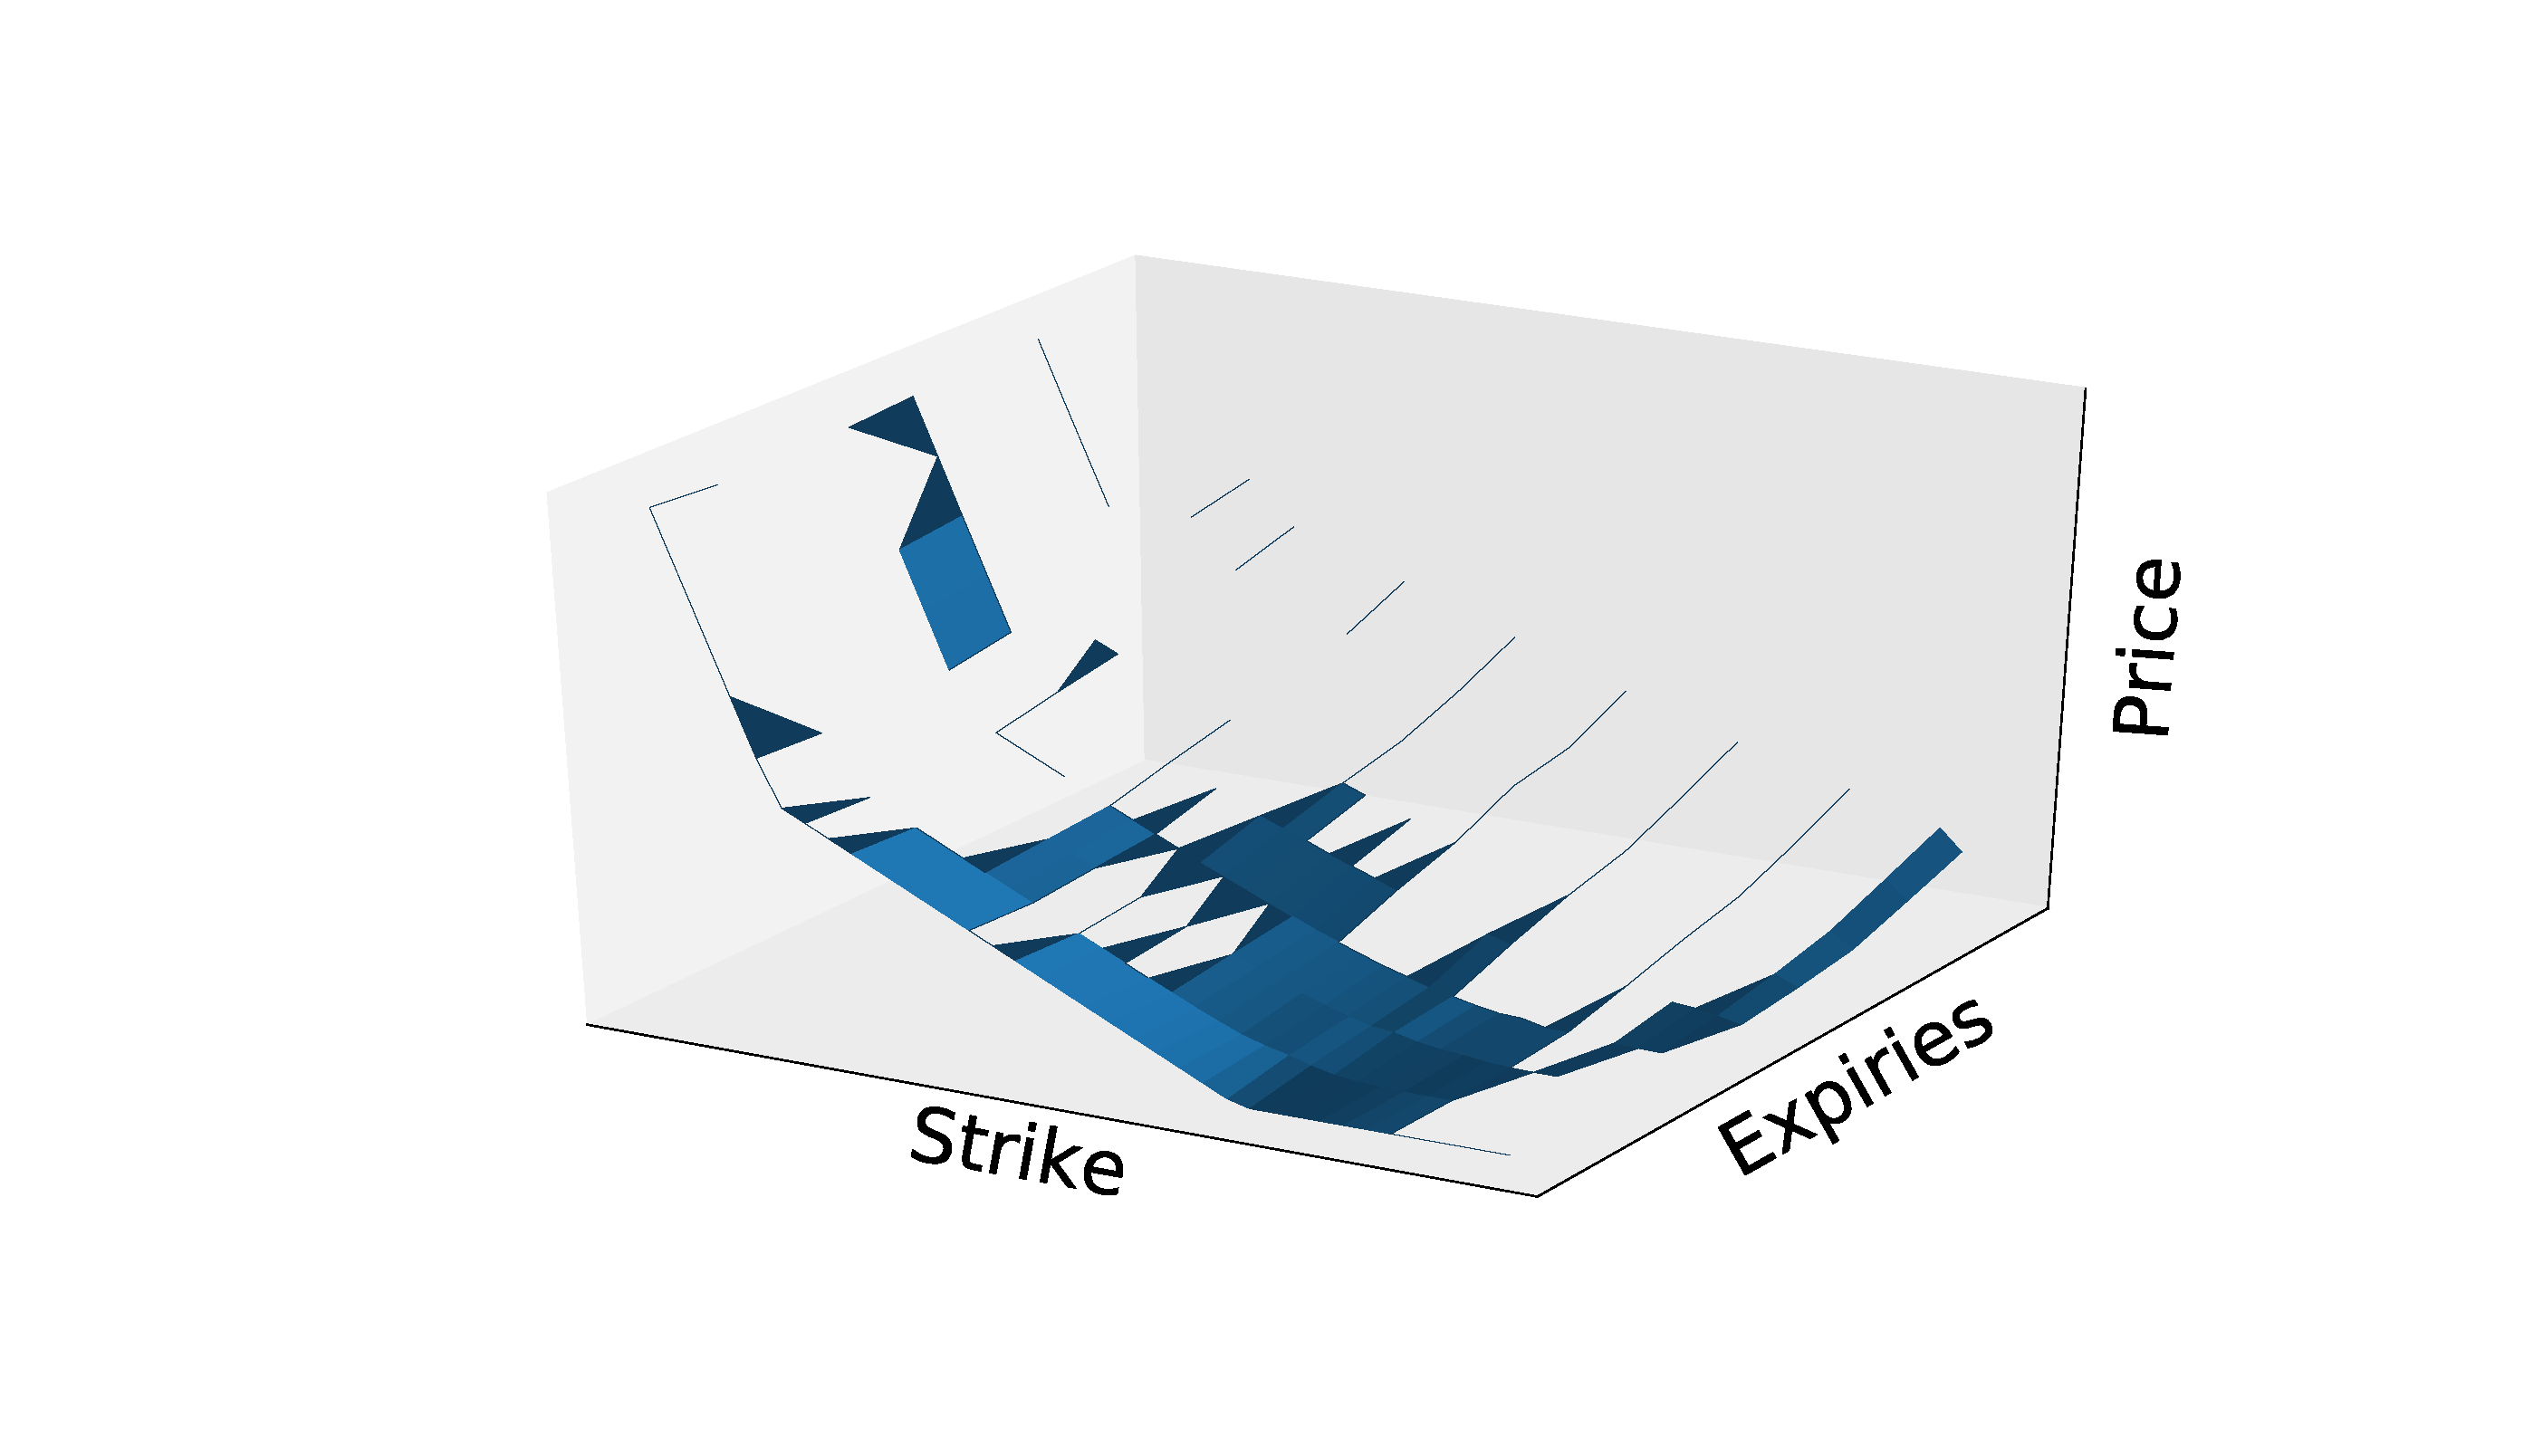
\includegraphics[width=\textwidth]{surf1}
		\caption{Before}
	\end{subfigure}
	\begin{subfigure}[b]{0.49\textwidth}
		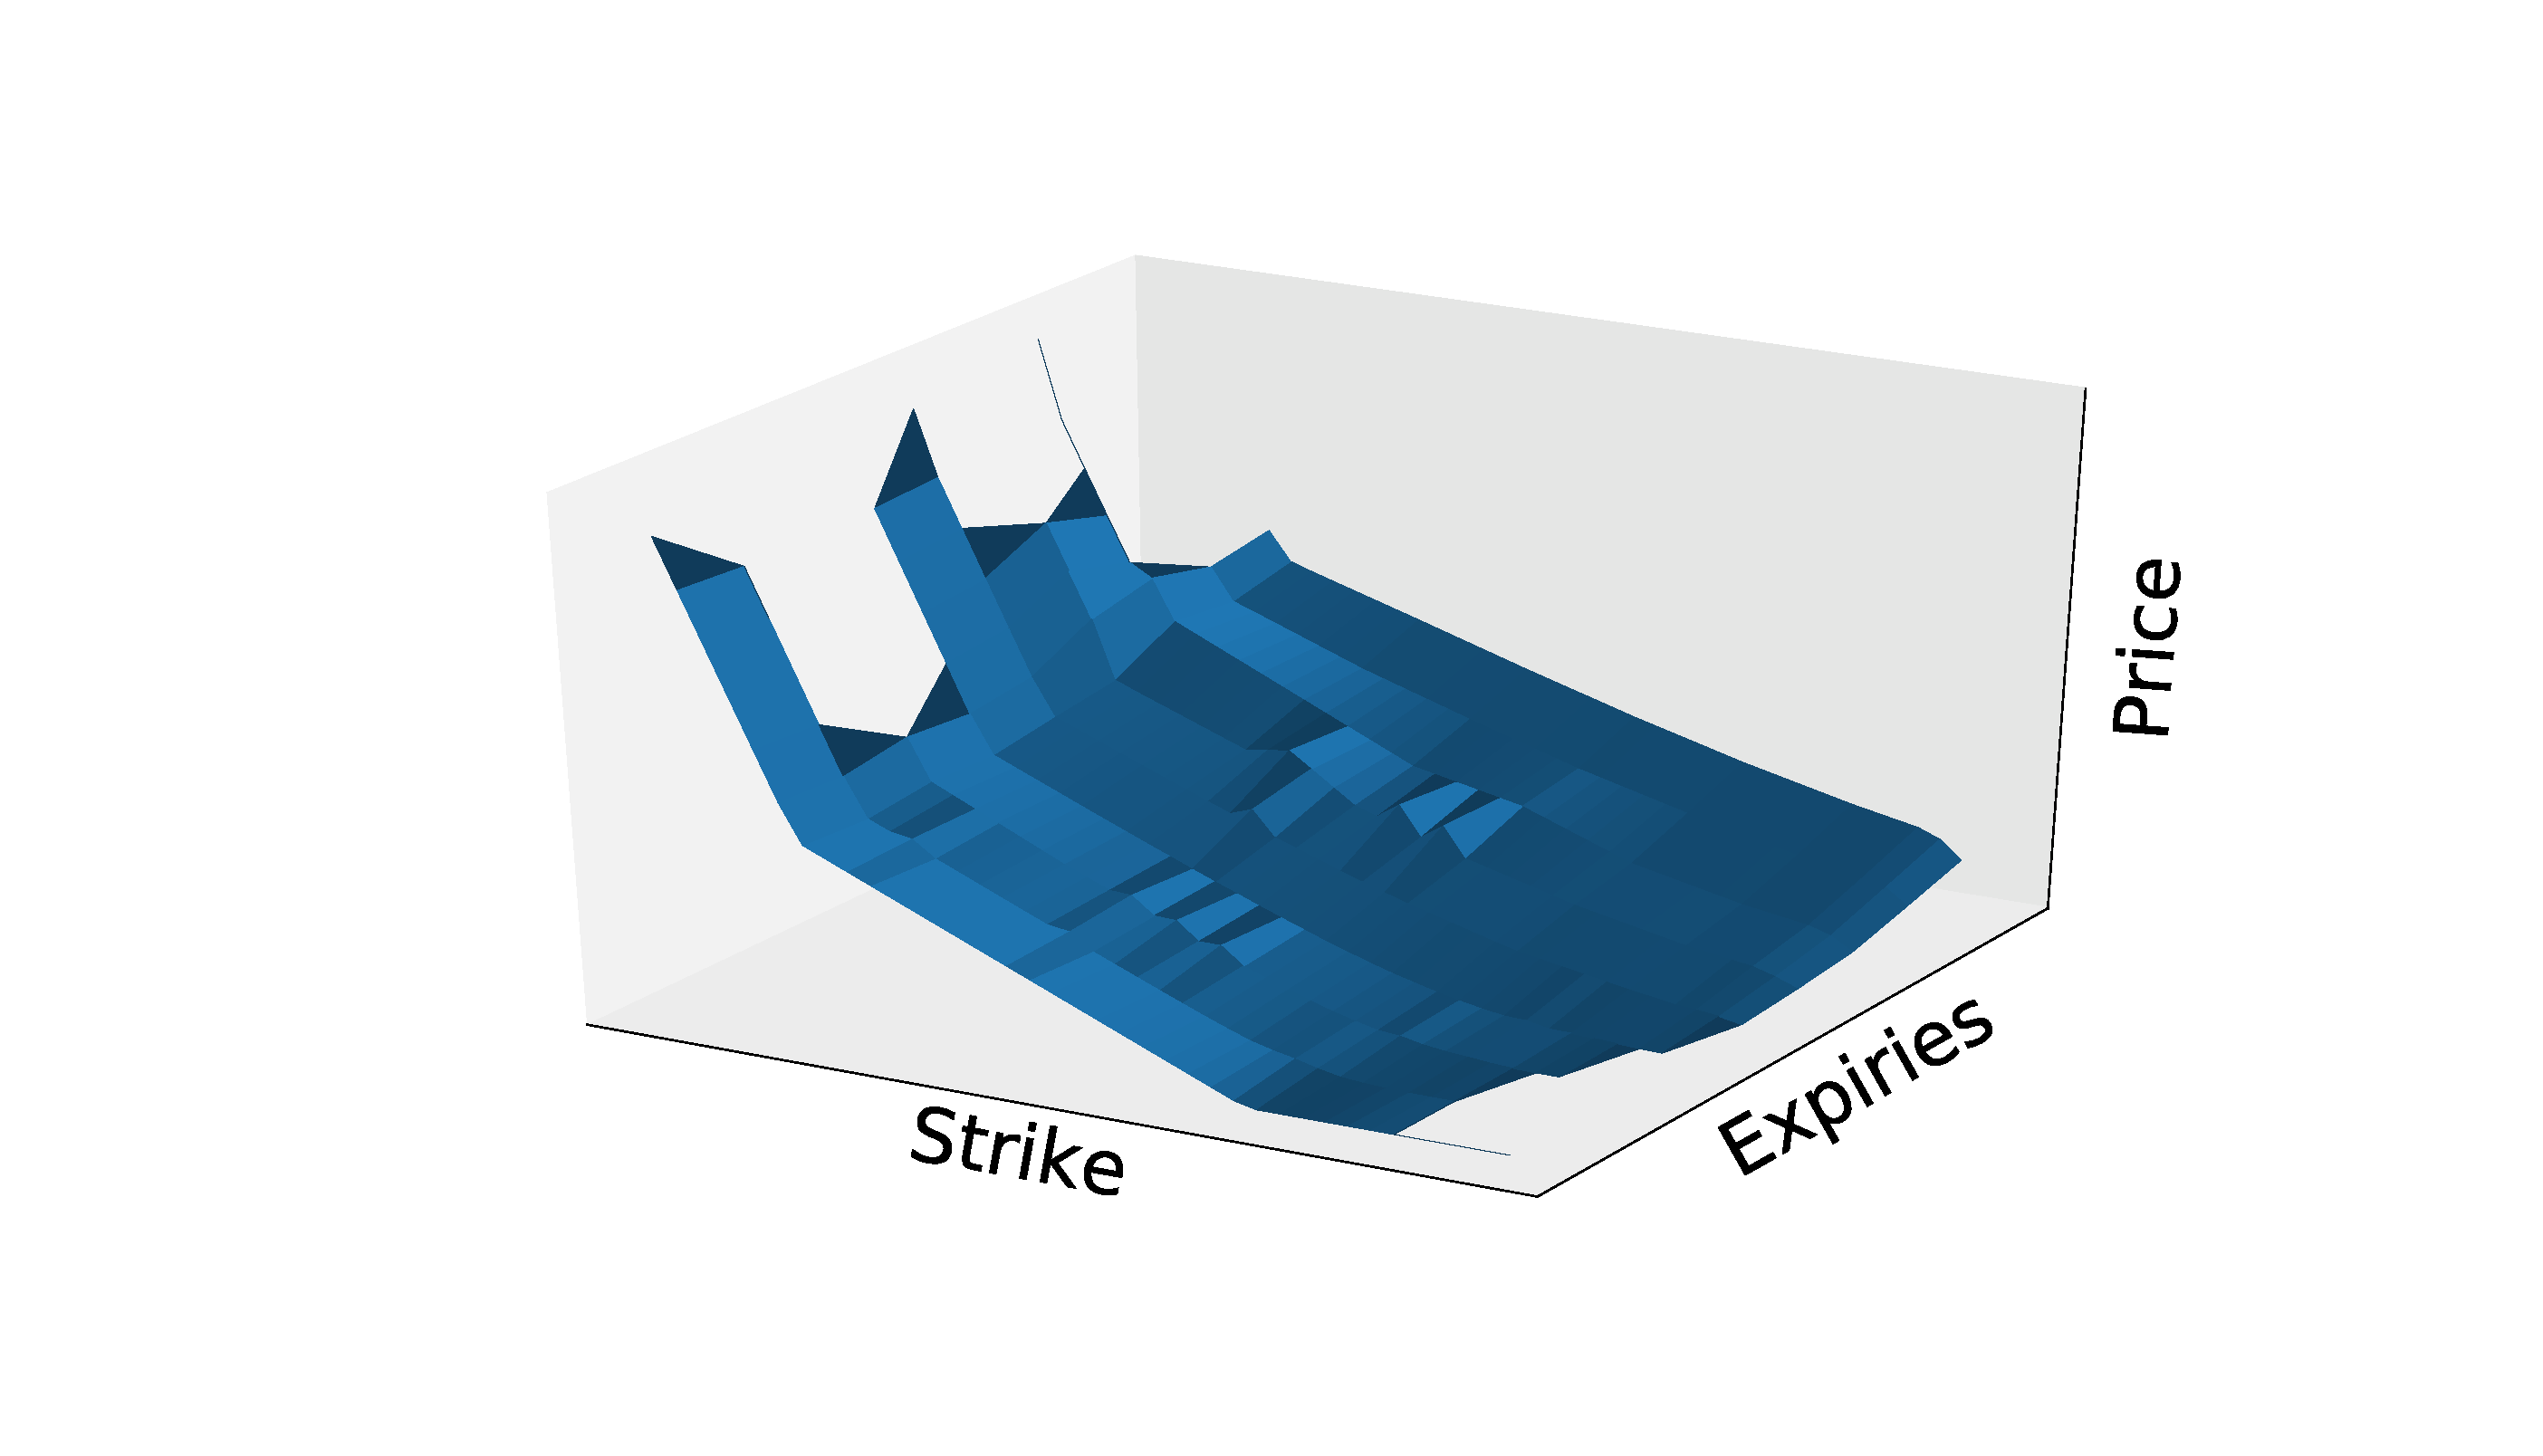
\includegraphics[width=\textwidth]{surf2}
		\caption{After}
	\end{subfigure}
	\caption{Illustration of Constructing a Price Surface}
\end{figure}
\footnotetext[7]{Jesper Andreasen and Brian Huge. "Volatility interpolation." Risk, 24(3):76, 2011.}
\end{frame}

\begin{frame}{Dupire’s forward equation}
\begin{itemize}
\item The forward price of a call option for delivery at time T:	$C(T,K)$
\item The spot price at t is: $C(T,K) e^{-\int^T_t r(s)ds}$.
\item It can be shown that :
\[
\frac{\partial C(T,K)}{\partial T}=\frac{1}{2} {\sigma}^2(T,K)K^2  \frac{\partial^2 C(T,K)}{ \partial K^2}
\]
\end{itemize}
\end{frame}




\begin{frame}{Model Calibration}
We can write finite difference  discretization of the Dupure forward equation as:
\[M\begin{bmatrix}
C(T_{i},K_0)\\
C(T_{i},K_1)\\
C(T_{i},K_2)\\
\vdots\\
C(T_{i},K_{n-1}) \\
C(T_{i},K_{n})
\end{bmatrix}=
\begin{bmatrix}
C(T_{i+1},K_0)\\
C(T_{i+1},K_1)\\
C(T_{i+1},K_2)\\
\vdots\\
C(T_{i+1},K_{n-1}) \\
C(T_{i+1},K_{n})
\end{bmatrix}
\]
We try to find $M$ that so that $C(T_{i+1},K_j)=C_{mkt}(T_{i+1},K_j)$. This can be done by:
\[
\inf_{\sigma(T_i,.)} \sum_{j}(\frac{C(T_{i+1},K_j)-C_{mkt}(T_{i+1},K_j)}{Vega_{bs}^{mkt}(T_{i+1},K_j)})^2
\]
Note that, for each $T_i$, we solve a separate optimization.  
\end{frame}


\begin{frame}{Interpolation Over  the Domain of Expiries}
After optimization,  the local volatility functions are translated into arbitrage-consistent prices for a discrete set of expiries but it does not
directly specify the option prices between the expiries. We can fill in the gaps by:
\[
\frac{C(T,K) -C(T_{i},K)}{T-T_{i}}=\frac{1}{2}\sigma(T_i,K)^2 K^2 \frac{\partial^2 C(T_{i+1},K) }  {\partial K^2} , T \in [T_i,T_{i+1})
\]
\end{frame}
\begin{frame}{Benefits of Interpolation Based On Local Vol Model}
Interpolation based on the above procedure can guarantee the option price given by interpolation is arbitrage-free:
\begin{enumerate}
\item No call spread arbitrage:
\[
\frac{\partial C(T,K)}{ \partial K} \leq 0
\]
\item  No butterfly spread arbitrage:
\[
\frac{\partial^2 C(T,K)}{ \partial K^2} \geq 0
\]
\item  No calendar spread arbitrage:
\[
\frac{\partial C(T,K)}{ \partial T} \geq 0
\]
\end{enumerate}
\end{frame}


\subsection{Real Data Experiments}
\begin{frame}[fragile]{Total Hedging Model for Real Data Case}
\begin{figure}[htp!]
	\centering
	\resizebox{0.90\textwidth}{!}{
		\begin{tikzpicture}[
		prod/.style={circle, draw, inner sep=0pt},
		ct/.style={circle, draw, inner sep=5pt, ultra thick, minimum width=10mm},
		ft/.style={circle, draw, minimum width=8mm, inner sep=1pt},
		filter/.style={circle, draw, minimum width=7mm, inner sep=1pt, path picture={\draw[thick, rounded corners] (path picture bounding box.center)--++(65:2mm)--++(0:1mm);
				\draw[thick, rounded corners] (path picture bounding box.center)--++(245:2mm)--++(180:1mm);}},
		mylabel/.style={font=\scriptsize\sffamily},
		>=LaTeX
		]
		%		\node[draw,rectangle]  (ps1) at (4.5-8, -1) {softmax};
		%		\node[draw,rectangle]  (ps3) at (7.5-8, -1) {softmax};
		%		\node [draw,circle,inner sep=0pt] (prp1) at (3*1-8, -1) {$\times$};
		%		\node  (prp2) at (3*2-8, -1.5) {$\dots$};
		%		\node [draw,circle,inner sep=0pt] (prp3) at (3*3-8, -1) {$\times$};
		
		%		\foreach \i [count=\step from 1] in {$\vx_1^P$,$\dots$,$\vx_O^P$}
		%		\node (pri\step) at (3*\step-8, -2) {\i};
		%		\node  (psw1) at (4.5-8, -2) {$SW_P$};
		%		\node  (psw3) at (7.5-8, -2) {$SW_P$};
		%		\draw[->] (ps1.west) to node[below]{$\mathbf{\beta}$} (prp1.east);
		%		\draw[->] (ps3.east) to node[below]{$\mathbf{\beta}$} (prp3.west);
		%		\draw[->] (pri1.north) to (prp1.south);
		%		\draw[->] (pri3.north) to (prp3.south);
		%		\draw[->] (psw1.north) to (ps1.south);
		%		\draw[->] (psw3.north) to (ps3.south);
		%		\node (ph2) at (3*2-8, 0.0) {$\dots$};
		%		\foreach \step in {1,3} {
		%			\node[draw,rectangle] (ph\step) at (3*\step-8, 0.0) {GRU};
		%		}
		%		\draw[->] (prp1.north) to node[left]{$\widehat{\vx}_1^P$} (ph1.south);
		%		\draw[->] (prp3.north) to node[left]{$\widehat{\vx}_O^P$} (ph3.south);
		%				
		%		\foreach \step in {1,...,2} {
		%			\pgfmathtruncatemacro{\next}{add(\step,1)}
		%			\draw[->] (ph\step.east) -> (ph\next.west);
		%		}
		%		\node[fit=(pri1) (pri3) (ps1) (ps3) (ph1) (ph3), draw, inner sep=0pt] (fit1) { };
		%		\node[align=center, outer sep=0] (encoder) [left=of fit1] {Local Hedging \\ Encoder};
		
		
		
		\node[filter] (poe2) at (9-7, 4.5) {};
		\node[filter] (poe3) at (6-7, 4.5) {};
		\node [draw,circle,inner sep=0pt] (poe4) at (6-7, 5.5) {$\times$};
		\node [draw,circle,inner sep=0pt] (poe5) at (9-7, 5.5) {$\times$};
		\node [draw,circle,inner sep=0pt] (poe6) at (7.5-7, 6) {$+$};
		\node (poe7) at (7.5-7, 7) {$V^M_{t_0}$};
		\node  (pbs) at (4.5-7, 5.5) {$V^{mkt}_{t_0}$};
		\draw[->] (poe3.north) to node[left]{$1-o$} (poe4.south);
		\draw[->] (poe3.north) to node[above]{$o$} (poe5.west);
		\draw[->] (poe2.north) to node[left]{$\widehat{V}^M_{t_0}$} (poe5.south);
		\draw[->] (poe4.north) to node[left]{} (poe6.west);
		\draw[->] (poe5.north) to node[left]{} (poe6.east);
		\draw[->] (poe6.north) to node[left]{} (poe7.south);
		\draw[->] (pbs.east) to node[left]{} (poe4.west);
		
		
		\draw[->] (poe7.east) to node[left]{} (loss.west);
		
		
		\node[draw,circle,inner sep=0pt]  (pl1) at (7.5-7, 2) {$\times$};
		\node[draw,rectangle]  (pl3) at (7.5-7, 1) {softmax};
		\node  (pl2) at (6-7, 2) {$\vy_P$};
		\node  (pl4) at (6-7, 1) {$LW_P$};
		\draw[->] (pl4.east) to (pl3.west);
		\draw[->] (pl2.east) to (pl1.west);
		\draw[->] (pl3.north) to node[left]{$\eta$} (pl1.south);
		
		
		\node (phe2) at (7.5-8, 3) {$\widehat{\vy}_P$};
		%		\node (phe3) at (9-8, 3) {$\widehat{\mathbf{h}}_E^P$};
		\draw[->] (pl1.north) to (phe2.south);
		%		\draw[->] (ph3.north) to  (phe3.south);
		%		\draw[->] (phe3.north) to  (poe2.south);
		%		\draw[->] (phe3.north) to  (poe3.south);
		
		\draw[->] (phe2.north) to (poe2.south);
		\draw[->] (phe2.north) to (poe3.south);
		
		\node[fit=(poe2) (poe3) (poe5) (poe6)  (pbs) (phe2) (pl3), draw, inner sep=4pt] (fit3) { };
		\node[align=center, outer sep=0] (encoder) [below=of fit3] {\Large Pricing Model};
		
		
		
		
		
		
		\node[draw,rectangle]  (s1) at (4.5, -1) {softmax};
		\node[draw,rectangle]  (s3) at (7.5, -1) {softmax};
		\node [draw,circle,inner sep=0pt] (rp1) at (3*1, -1) {$\times$};
		\node  (rp2) at (3*2, -1.5) {$\dots$};
		\node [draw,circle,inner sep=0pt] (rp3) at (3*3, -1) {$\times$};
		
		\foreach \i [count=\step from 1] in {$\vx_1^{t_i}$,$\dots$,$\vx_K^{t_i}$}
		\node (ri\step) at (3*\step, -2) {\i};
		\node  (sw1) at (4.5, -2) {SW};
		\node  (sw3) at (7.5, -2) {SW};
		\draw[->] (s1.west) to node[below]{$\mathbf{\alpha}$} (rp1.east);
		\draw[->] (s3.east) to node[below]{$\mathbf{\alpha}$} (rp3.west);
		\draw[->] (ri1.north) to (rp1.south);
		\draw[->] (ri3.north) to (rp3.south);
		\draw[->] (sw1.north) to (s1.south);
		\draw[->] (sw3.north) to (s3.south);
		\node (h2) at (3*2, 0.0) {$\dots$};
		\foreach \step in {1,3} {
			\node[draw,rectangle] (h\step) at (3*\step, 0.0) {GRU};
		}
		\draw[->] (rp1.north) to node[left]{$\widehat{\vx}_1^{t_i}$} (h1.south);
		\draw[->] (rp3.north) to node[left]{$\widehat{\vx}_K^{t_i}$} (h3.south);
		
		\foreach \step in {1,...,2} {
			\pgfmathtruncatemacro{\next}{add(\step,1)}
			\draw[->] (h\step.east) -> (h\next.west);
		}
		\node[fit=(ri1) (ri3) (s1) (s3) (h1) (h3), draw, inner sep=0pt] (fit4) { };
		%\node[align=center, outer sep=0] (encoder) [right=of fit4] {Hedging \\Encoder};
		\node[draw,circle,inner sep=0pt]  (l1) at (6, 2) {$\times$};
		\node[draw,rectangle]  (l3) at (6, 1) {softmax};
		\node  (l2) at (4.5, 2) {$\vy_{t_i}$};
		\node  (l4) at (4.5, 1) {$LW$};
		\draw[->] (l4.east) to (l3.west);
		\draw[->] (l2.east) to (l1.west);
		\draw[->] (l3.north) to node[left]{$\omega$} (l1.south);
		\node (he2) at (6, 3) {$\widehat{\vy}_{t_i}$};
		\node (he3) at (9, 3) {$\widehat{\mathbf{h}}_E^{t_i}$};
		\node[fit=(he2) (he3), draw, inner sep=0pt] (fit6) { };
		\node[draw,rectangle]  (hedge) at (7.5, 4) {GRU};
		\node[filter](output) at (7.5, 5) {};
		\node[draw,rectangle] (loss) at (7.5, 7) {Loss};
		%        \node (V0) at (7.5, 8) {$V_{t_0}$};
		\node  (outputPre) at (6, 5) {...};
		\node  (outputNext) at (9, 5) {...};
		\node  (hedgePre) at (6, 4) {...};
		\node (hedgeNext) at (9, 4) {...};
		
		
		
		
		\node[draw,rectangle]  (hedge0) at (4.5, 4) {GRU};
		\node[filter](output0) at (4.5, 5) {};
		\node[draw,rectangle]  (hedgeF) at (10.5, 4) {GRU};
		\node[filter](outputF) at (10.5, 5) {};
		\draw[->] (l1.north) -> (he2.south);
		\draw[->] (h3.north) -> (he3.south);
		\draw[->] (he2.north) -> (hedge.south);
		\draw[->] (he3.north) -> (hedge.south);
		%\draw[->] (V0.south) -> (loss.north);
		\draw[->] (hedge0.east) -> (hedgePre.west);
		\draw[->] (hedgeNext.east) -> (hedgeF.west);
		
		\draw[->] (hedge.north) to node[left]{${\mathbf{c}}_{t_i}$} (output.south);
		\draw[->] (hedge.north) to node[left]{${\mathbf{c}}_{t_i}$} (output.south);
		
		\draw[->] (hedge0.north) to node[left]{${\mathbf{c}}_{t_0}$} (output0.south);
		\draw[->] (hedgeF.north) to node[left]{${\mathbf{c}}_{t_{N-1}}$} (outputF.south);
		
		\draw[->] (hedgePre.east) to  (hedge.west);
		\draw[->] (hedge.east) to (hedgeNext.west);
		
		\node[fit=(hedge) (hedge0) (hedgeF) (output0) (output) (outputF), draw, inner sep=0pt] (fit5) { };
		\node[align=center, outer sep=0] (encoder) [below=of fit4] { \Large Total hedging Model};
		\node[rectangle]  (delta0) at (4.5, 6) {$\delta_{t_0}$};
		\node[rectangle]  (deltaP) at (6, 6) {...};
		\node[rectangle]  (delta) at (7.5, 6) {$\delta_{t_i}$};
		\node[rectangle]  (deltaN) at (9, 6) {...};
		\node[rectangle]  (deltaF) at (10.5, 6) {$\delta_{t_{N-1}}$};
		\draw[->] (delta0.north) -> (loss.south);
		\draw[->] (deltaP.north) -> (loss.south);
		\draw[->] (delta.north) -> (loss.south);
		\draw[->] (deltaN.north) -> (loss.south);
		\draw[->] (deltaF.north) -> (loss.south);
		\draw[->] (output0.north) -> (delta0.south);
		\draw[->] (output.north) -> (delta.south);
		\draw[->] (outputF.north) -> (deltaF.south);
		
		
		
		
		
		
		
		
		
		%\node[draw,rectangle]  (ls1) at (4.5+10, -1) {softmax};
		%\node[draw,rectangle]  (ls3) at (7.5+10, -1) {softmax};
		%\node [draw,circle,inner sep=0pt] (lrp1) at (3*1+10, -1) {$\times$};
		%\node  (lrp2) at (3*2, -1.5) {$\dots$};
		%\node [draw,circle,inner sep=0pt] (lrp3) at (3*3+10, -1) {$\times$};
		%
		%\foreach \i [count=\step from 1] in {$\vx_1$,$\dots$,$\vx_N$}
		%\node (lri\step) at (3*\step+10, -2) {\i};
		%\node  (lsw1) at (4.5+10, -2) {SW};
		%\node  (lsw3) at (7.5+10, -2) {SW};
		%\draw[->] (ls1.west) to node[below]{$\mathbf{\alpha}$} (lrp1.east);
		%\draw[->] (ls3.east) to node[below]{$\mathbf{\alpha}$} (lrp3.west);
		%\draw[->] (lri1.north) to (lrp1.south);
		%\draw[->] (lri3.north) to (lrp3.south);
		%\draw[->] (lsw1.north) to (ls1.south);
		%\draw[->] (lsw3.north) to (ls3.south);
		%\node (lh2) at (3*2+10, 0.0) {$\dots$};
		%\foreach \step in {1,3} {
		%	\node[draw,rectangle] (lh\step) at (3*\step+10, 0.0) {GRU};
		%}
		%\draw[->] (lrp1.north) to node[left]{$\hat{\vx}_1$} (lh1.south);
		%\draw[->] (lrp3.north) to node[left]{$\hat{\vx}_N$} (lh3.south);
		%
		%%\draw[->] (i4) -> (h4.south);
		%
		%\foreach \step in {1,2} {
		%	\pgfmathtruncatemacro{\next}{add(\step,1)}
		%	\draw[->] (lh\step.east) -> (lh\next.west);
		%}
		%%\node[fit=(lri1) (lri3) (ls1) (ls3) (h1) (h3), draw, inner sep=0pt] (fit1) { };
		%%\node[align=center, outer sep=0] (encoder) [right=of fit1] {Encoder};
		
		
		
		\node[filter] (loe2) at (9+7, 4.5) {};
		\node[filter] (loe3) at (6+7, 4.5) {};
		\node [draw,circle,inner sep=0pt] (loe4) at (6+7, 5.5) {$\times$};
		\node [draw,circle,inner sep=0pt] (loe5) at (9+7, 5.5) {$\times$};
		\node [draw,circle,inner sep=0pt] (loe6) at (7.5+7, 6.5) {$+$};
		\node (loe7) at (7.5+7, 7.5) {$\delta_L^{t_i}$};
		\node  (lbs) at (10+7, 5.5) {$\delta_{BS}^{t_i}$};
		\draw[->] (loe3.north) to node[left]{$\widehat{\delta_L}^{t_i}$} (loe4.south);
		\draw[->] (loe2.north) to node[above]{$o$} (loe4.east);
		\draw[->] (loe2.north) to node[right]{$1-o$} (loe5.south);
		\draw[->] (loe4.north) to node[left]{} (loe6.west);
		\draw[->] (loe5.north) to node[left]{} (loe6.east);
		\draw[->] (loe6.north) to node[left]{} (loe7.south);
		\draw[->] (lbs.west) to node[left]{} (loe5.east);
		
		\draw [->]  (deltaP.east) to[out=0,in=180] (hedge.west);
		\draw [->]  (delta0.east) to[out=0,in=180] (hedgePre.west);
		\draw [->]  (delta.east) to[out=0,in=180] (hedgeNext.west);	
		\draw [->]  (deltaN.east) to[out=0,in=180] (hedgeF.west);	
		
		
		%\node[draw,circle,inner sep=0pt]  (ll1) at (6+10, 2) {$\times$};
		%\node[draw,rectangle]  (ll3) at (6+10, 1) {softmax};
		%\node  (ll2) at (4.5+10, 2) {$\vx_L$};
		%\node  (ll4) at (4.5+10, 1) {$LW$};
		%\draw[->] (ll4.east) to (ll3.west);
		%\draw[->] (ll2.east) to (ll1.west);
		%\draw[->] (ll3.north) to node[left]{$\omega$} (ll1.south);
		
		
		\node (lhe2) at (6+7, 3) {$\widehat{\vy}_{t_i}$};
		\node (lhe3) at (9+7, 3) {$\hat{\mathbf{h}}_E^{t_i}$};
		%\draw[->] (ll1.north) to (lhe2.south);
		%\draw[->] (lh3.north) to  (lhe3.south);
		\draw[->] (lhe3.north) to  (loe2.south);
		\draw[->] (lhe3.north) to  (loe3.south);
		
		\draw[->] (lhe2.north) to (loe2.south);
		\draw[->] (lhe2.north) to (loe3.south);
		\node[fit=(lhe2) (lhe3), draw, inner sep=0pt] (fit7) { };
		\node[align=center, outer sep=0] (encoder) [below=of fit7] { \Large Local hedging model};
		\draw[->] (fit6) to (fit7);
		%\node[fit=(loe2) (loe3) (loe5) (loe6)  (loe7)  (lbs) (lhe2) (lhe3) (lh1) (lh3) (lri1) (lri3), draw, inner sep=4pt] (fit3) { };
		%\node[align=center, outer sep=0] (encoder) [below=of fit3] {Local hedging model};
		%\draw[->] (fit3) -> (he3.east);
		
		
		
		\end{tikzpicture}
	}
	\caption{Refined Model For Real Cases}
	\label{fig:RNNModel}
\end{figure}
\end{frame}

\begin{frame}{Primitive Experimental Setting}
\begin{itemize}
	\item Testing period is from 2007 and 2014 for SP500 index option.
	\item Scenario: weekly hedging for two months.
	\item All data in previous years is used as training.
	\item Model are updated yearly.
	\item Early stopping is used as regulation
	\item Performance is evaluated with \textbf{relative} hedging error.
	\[ 
	rel_{err}=\frac{P^i_{t_N^-}}{V_{t_0}}
	\]
\end{itemize}
\end{frame}

\begin{frame}{Value-At-Risk of \textbf{Relative} Hedging Error}
\begin{table}[htp!]
	\centering
\begin{tabular}{|c|c|c|c|}
	\hline
	% after \\: \hline or \cline{col1-col2} \cline{col3-col4} ...
	method &Total&Local&BS \\
	2007&\textbf{-0.8622}&-1.044&-2.3724\\
	2008&\textbf{-1.1430}&-1.0782&-4.9241\\
	2009&\textbf{-0.4563}&-1.3607&-2.3771\\
	2010&\textbf{-0.4509}&-0.6817&-1.7911\\
	2011&\textbf{-0.7062}&-0.9049&-1.9094\\
	2012&\textbf{-0.3866}&-1.7635&-2.6473\\
	2013&\textbf{-0.4635}&-2.7910&-4.2887\\
	2014&\textbf{-1.5424}&-2.0567&-3.1884\\
	\hline
\end{tabular}

	\caption{Value-At-Risk}
\end{table}

\end{frame}




\begin{frame}{Expected Shortfall of \textbf{Relative} Hedging Error}
\begin{table}[htp!]
	\centering
		\begin{tabular}{|c|c|c|c|}
		\hline
		% after \\: \hline or \cline{col1-col2} \cline{col3-col4} ...
		method &Total&Local&BS \\
		2007&\textbf{-1.1568}&-1.8545&-5.4942\\
		2008&\textbf{-2.0683}&-4.9241&-7.3248\\
		2009&\textbf{-0.6443}&-2.3772&-5.0323\\
		2010&\textbf{-0.6207}&-1.1806&-3.6964\\
		2011&\textbf{-1.1439}&-1.9460&-3.2358\\
		2012&\textbf{-0.5497}&-3.2662&-4.7711\\
		2013&\textbf{-0.6460}&-4.3091&-6.6587\\
		2014&\textbf{-1.9005}&-3.4671&-5.2354\\
		\hline
	\end{tabular}
	
	\caption{Expected Shortfall}
\end{table}
\end{frame}

\begin{frame}{Mean Absolute \textbf{Relative} Hedging Error}
\begin{table}[htp!]
	\centering
	
	\begin{tabular}{|c|c|c|c|}
		\hline
		% after \\: \hline or \cline{col1-col2} \cline{col3-col4} ...
		method &Total&Local&BS \\
		2007&\textbf{0.3769}&0.7357&1.3396\\
		2008&\textbf{0.5034}&0.6852&0.9068\\
		2009&\textbf{0.3041}&0.6597&0.5092\\
		2010&\textbf{0.3412}&0.5837&1.1331\\
		2011&\textbf{0.3507}&0.4611&0.8513\\
		2012&\textbf{0.2726}&0.5858&0.8084\\
		2013&\textbf{0.3055}&0.8961&0.9710\\
		2014&\textbf{0.5876}&0.9509&1.6091\\
		\hline
	\end{tabular}
	\caption{Mean Absolute \textbf{Relative} Hedging Error}
\end{table}

\end{frame}

\begin{frame}{Standard Deviation of \textbf{Relative} Hedging Error}
\begin{table}[htp!]
	\centering
	
	\begin{tabular}{|c|c|c|c|}
		\hline
		% after \\: \hline or \cline{col1-col2} \cline{col3-col4} ...
		method &Total&Local&BS \\
		2007&\textbf{0.4977}&2.2085&3.2548\\
		2008&\textbf{0.7645}&2.4953&3.7674\\
		2009&\textbf{0.3785}&1.3938&2.6829\\
		2010&\textbf{0.4770}&1.1388&1.3975\\
		2011&\textbf{0.4787}&0.7269&1.1465\\
		2012&\textbf{0.3339}&0.9633&1.5448\\
		2013&\textbf{0.3717}&1.4185&2.6968\\
		2014&\textbf{0.8899}&2.2879&5.3217\\
		\hline
	\end{tabular}
	\caption{Standard Deviation}
\end{table}
\end{frame}
\begin{frame}{Q \& A}
\LARGE
\begin{quote}
	\alert{Thank you very much!}\\
	\hspace{8ex} Any Questions?
\end{quote}
\end{frame}

\end{document}

